\chapter{Introducción: La neorreación devela la crisis del Estado moderno}
\label{cha:la-neorreación-devela-la-crisis-del-estado-moderno}

\epigraph{\enquote{Bajo tal mirada esta época nuestra puede ser llamada \enquote{época de ilustración} o también \enquote{el Siglo de Federico}}}{\emph{Immanuel Kant} en~\autocite[p.~11]{kantQueEsIlustracion2009}.}

Nuestro tiempo es de implacable ironía y de un cinismo cada vez más vacío. Mientras el proyecto de la Ilustración, gran promesa de los fundadores del Estado moderno, se derrite, las resistencias se refugian en formas de activismo poco capaces de transformar la realidad a escala molar, global. \footnote{Estos conceptos se refieren a una escala local, micro y global o macro, respectivamente Desde el vocabulario deleuziano son denominaciones comunes a este aparente binarismo.} La derecha alternativa llama a estos refugios de autocomplacencia \enquote{Catedrales}, un espacio seguro para el sentimentalismo y la camaradería de las minorías, incluyendo a una que otra persona que goza del estatuto verdadero de ciudadana y que deserta para alcanzar el \emph{tiqqun}, la redención. Los mismos hombres-masa resentidos llenan internet de propaganda que toma partido por la Ilustración tal y como la entendía el despotismo ilustrado de \enquote{hombres de Estado} como Federico el Grande.

Mientras, cualquier intento de imaginación política ha sido cooptado por el neoliberalismo, un momento histórico del capital donde el mercado tiene un producto para complacer a cualquiera. El desarrollo de la cibernética y el creciente poder de las corporaciones como entidades transnacionales inunda a cualquier discurso político de un montón de limitaciones económicas por un hecho fundamental: mientras las estructuras tecnológicas sean dominadas por la lógica privativa del capital, nunca será posible encontrar un afuera a la religión de Estado, pues la tecnología no solo condiciona nuestras capacidades tecnomateriales sino que también captura nuestro deseo e inunda nuestra avida psíquica.

En la \emph{Introducción a la guerra civil}, el Comité Invisible señala que la guerra civil es el libre juego de las formas de vida, el principio de su coexistencia. \autocite[pág. 17]{tiqqunIntroduccionGuerraCivil2008}. De la guerra civil trata esta investigación. Pues, como señala Tiqqun, si las sociedades tradicionales conocían el robo, la blasfemia, el parricidio, el rapto, el sacrificio, la afrenta y la venganza, las sociedades modernas (al menos legalmente) creen en la violencia como lo que le es dado solo al Estado. La violencia, dicen en \emph{Tiqqun} es aquello de lo que hemos sido desposeídos, y aquello de lo que hace falta ahora reapropiarse. Sobre el argumento anterior se funda este trabajo.

\section{Según los neorreaccionarios, la Ilustración se derrite}
\label{sec:según-los-neorreaccionarios}

Observa la siguiente imagen:

\begin{figure}[!ht]
  \centering
  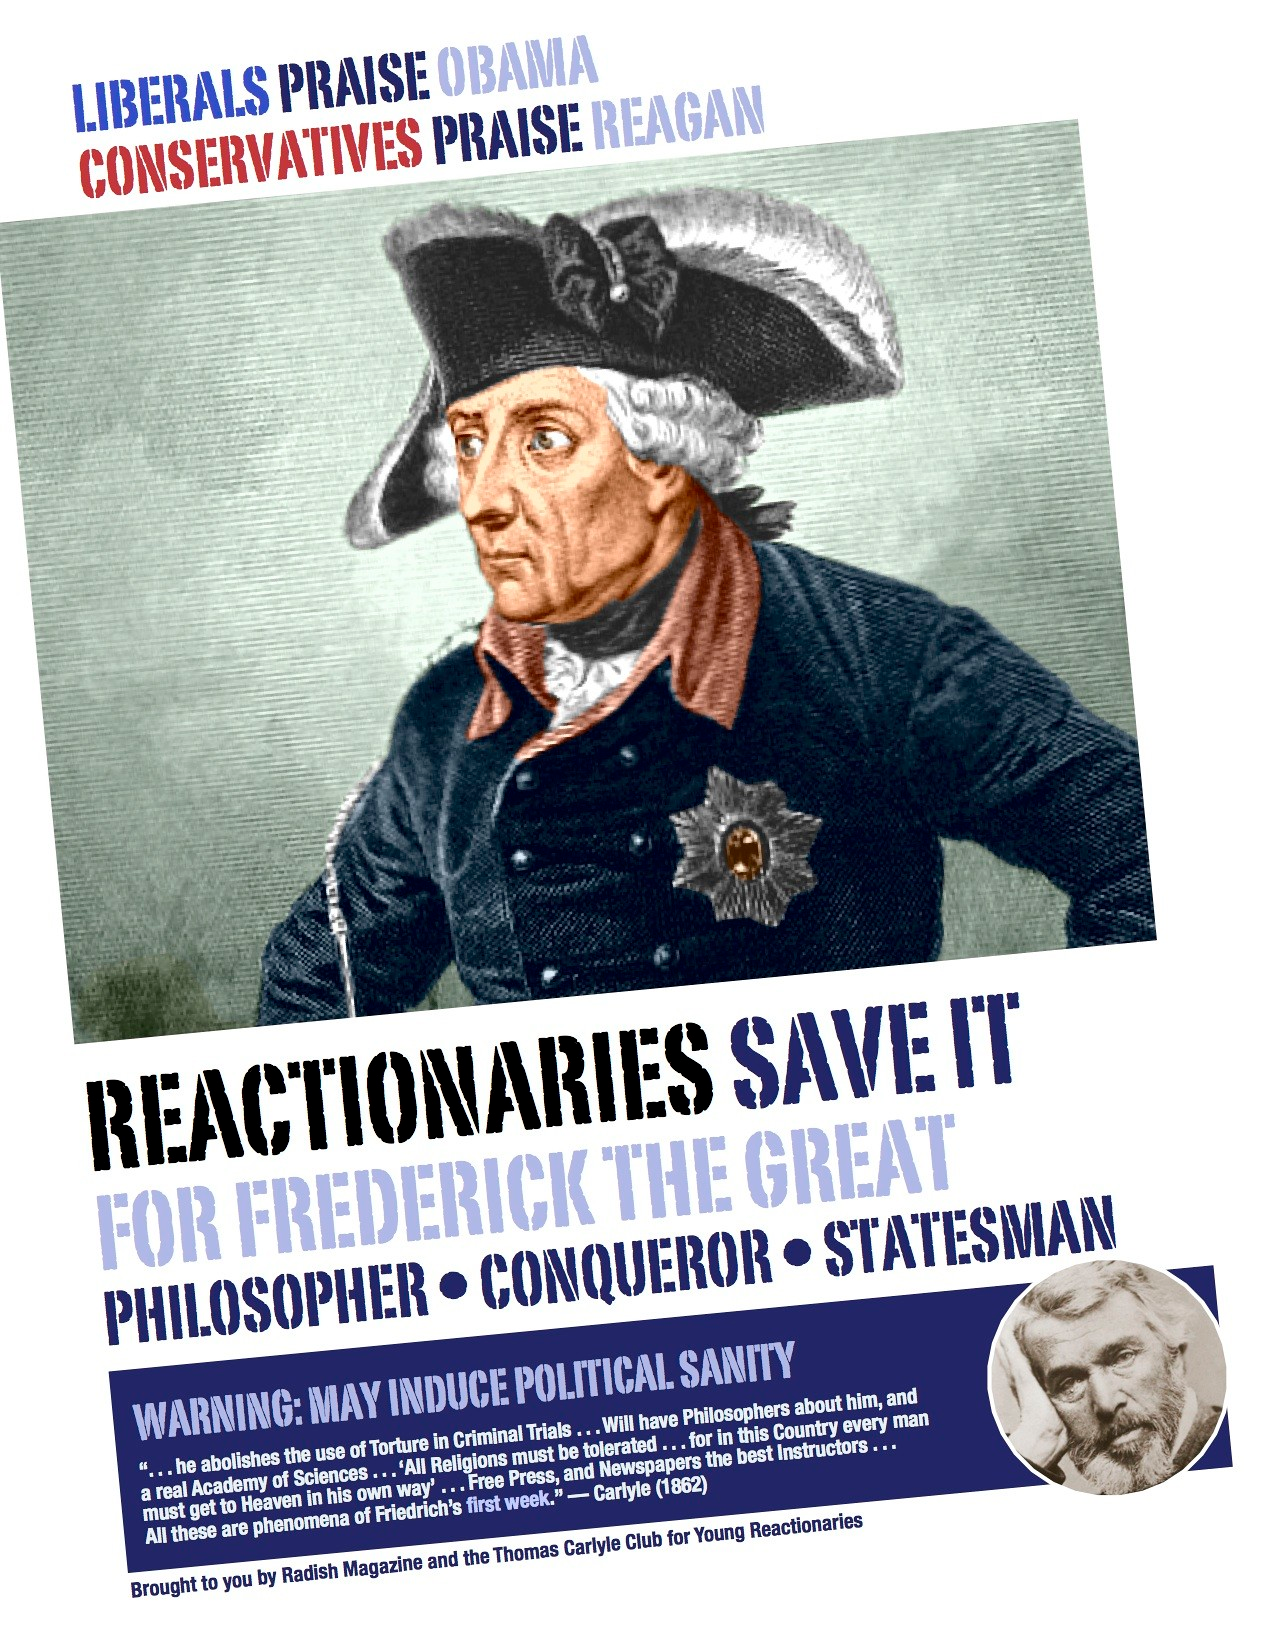
\includegraphics[width=0.7\linewidth]{images/carlyle-neorreactionaries.png}
  \caption{Federico el Grande en un cartel de propaganda neorreaccionaria}
  \label{fig:federico}
\end{figure}

En ella se aprecia el cartel propagandístico en inglés de un sitio web de Estados Unidos de América. Se mira a Federico el Grande con una leyenda que dice que, a diferencia de los liberales, que rezan a Obama, y de los conservadores, que lo hacen para Reagan, la visión neorreaccionaria simpatiza con Federico, rey alemán, filósofo, conquistador y hombre de Estado \autocite{huiUnhappyConsciousnessNeoreactionaries2017}. Los neorreaccionarios son un movimiento primordialmente compuesto por hombres blancos cisgénero en EUA, creen que mientras que la tecnología y el capitalismo han avanzado, la democracia ha obstaculizado el desarrollo económico, que para ellos constituye el \emph{telos} de las sociedades. Proponen un regreso al tradicionalismo en roles de género, jerarquías sociales y a la monarquía \autocite{AskphilosophyWhatNeoreactionarism}. Su posición virilista es la sublimación de resentimientos y de frustración sexual.

Los neorreaccionarios son emprendedores de alta tecnología de Sillicon Valley y su ideología política se proyecta la construcción de una utopía tecnocapitalista. Los neorreaccionarios son hombres resentidos, tristes, que pueden ver los problemas de los que son parte, pero hacen de la crítica un instrumento, y de la soberbia de sus pretensiones heroicas una ideología sobre La Razón. Son hombres enfermos de sospecha, pues todo les es dado a través del arreglo mercantil. Son ciborgs melancólicos, su potencia ha sido castrada por su conciencia de ser el ciudadano ideal, aquel por el que la explotación tiene sentido. No pueden imaginar un futuro afuera de la sociedad mercantil, desean \emph{desear el Estado}. Son el sujeto pleno de derecho, la promesa del Estado moderno. De ahí su frustración, de estar en el tope del privilegio, de su imposibilidad de morir. Su conciencia infeliz y su devenir cínico se manifiesta en su tono irónico. Viven en una tensión entre experiencia y concepto. Para los neorreaccionarios, la Ilustración es un otro alienado del yo, constituye un \emph{pharmakón}, remedio y veneno. El anacronismo y anti-intelectualismo son herramientas de los neorreaccionarios para construir un discurso donde la razón y la ciencia son concebidas para justificar el estado de las cosas. Feminizan los actos de resistencia de activistas para señalar el desvarío de la rabia y descalificar cualquier sublevación como irracional, como terrorismo que atenta contra la sociedad. Para los neorreaccionarios, la voluntad general es como el interés general: la Contradicción hegeliana del yo que se vuelve absoluto, una conciencia triste al saber que Dios ha muerto. De ahí que estos hombres tristes señalen que la \enquote{Catedral} es la iglesia contemporánea de la correctitud política. El síntoma de la conciencia infeliz del neorreaccionario se manifiesta a través de una ironía implacable \autocite{huiUnhappyConsciousnessNeoreactionaries2017}.

\begin{quote}
  \emph{La voluntad general como interés general: la Contradicción hegeliana del yo que se vuelve absoluto, una conciencia triste al saber que Dios ha muerto.}~\autocite{huiUnhappyConsciousnessNeoreactionaries2017}.
\end{quote}

Su apuesta por un regreso al absolutismo ilustrado es el síntoma de un proceso muy curioso en la Historia y de repercusiones políticas importantes. El \emph{meltdown}, concepto apropiado por los reaccionarios que puede traducirse como hundimiento o derretimiento, se refiere a la decadencia del proyecto de Ilustración y es también el título de una obra de Nick Land \autocite{landFangedNoumenaCollected2018}, es también síntoma de una crisis profunda en la civilización moderna que se manifiesta en la ecocatástrofe y el exterminio. Este vuelco a la política monárquica y al autoritarismo son parte de los movimientos de derecha en Estados Unidos cuyas ideas han creado organizaciones que buscan la toma del poder. Que el movimiento neorreaccionario tenga como polos a Donald Trump, empresario septuagenario, y a Pepe la Rana, meme que dio fama a la derecha alternativa \autocite{huiUnhappyConsciousnessNeoreactionaries2017} en el internet estadunidense, muestra dos caras de un mismo malestar en el Estado moderno. La llegada de Trump; el desarrollo altamente personalizado de la industria farmacopornográfica, régimen bio-molecular y semiótico-técnico de producción de subjetividad \autocite{preciadoTestoYonqui2008}; y el auge de foros de adolescentes encerrados en sus sótanos en el sitio web \url{4chan.org}; evidencian que la derecha alternativa se ha apoderado del gobierno del país más poderoso ---y endeudado--- del mundo. Este momento histórico evidencia una era poshistórica, posverdad, caracterizada por el derrumbamiento de la política iluminista de los Estados-nación, basada en la representación estética y racionalidad económica. La complejidad del contexto plantea grandes limitaciones teóricas a la academia de acceder a las raíces del problema.

\begin{figure}[htb]
  \centering
  
\includegraphics[width=0.7\linewidth]{images/pepe.jpg}
  \caption{\emph{Pepe the frog}, personaje de internet famoso por su uso en los memes.}
  \label{fig:pepe}
\end{figure}

La estética reaccionaria parece transgredir las convenciones de \hlfix{correctitud}{\ldots\ de \emph{corrección política} queda mejor.} política necesarias para considerarlo seriamente un movimiento político. Sin embargo, pese a la ambigüedad de sus postulados, los neorreaccionarios sienten melancolía por una idea de Occidente parecida al despotismo ilustrado que guiaría a la Humanidad al progreso. Para ellos, la cuestión de la productividad y la despolitización tecnocomercial son parte de lo necesario para salvar a Occidente. En el \ref{cha:el-rostro} ahondaré más en la cuestión del derretimiento causado, según este movimiento, por la democracia liberal.

\section{La política \emph{folk} es insuficiente para crear una alternativa}
\label{sec:la-política-folk}

\epigraph{Al enfatizar y permanecer en el ámbito de lo inmediato, la política \emph{folk} carece de las herramientas para transformar el neoliberalismo en otra cosa.}{\emph{Nick Srnićek} en~\autocite{srnicekInventarFuturoPoscapitalismo2017}.}

Tanto los movimientos radicales que están enamorados de la congruencia moral como los liberales, amantes del discurso tecnocientífico capitalista, son el síntoma de una intensa guerra de pensamientos que produce una interioridad psíquica hostil contra sí misma y contra la otredad. La guerra contra nuestro deseo y contra el mundo es un rasgo de lo que Tiqqun nombraría \emph{antropología positiva}, la captura de toda experiencia, de toda técnica, para el Capital. Nuestro deseo no es nuestro. Deseamos al Estado porque su operación principal es hacer que las formas de vida deseen deseo de Estado. En ese sentido es que el Estado moderno, epítome de la modernidad y de las fantasías detrás del concepto de Occidente que profesan los neorreaccionarios, es una religión.

La política folk es un concepto presente en las estrategias de guerra de los neorreaccionarios. Foros de internet de hombres blancos alienados que miran pornografía \emph{gore} dieron forma a los primeros memes del internet. En este contexto, internet se convirtió en una plataforma de debate político cuyos agentes fueron hombres resentidos con un alto capital tecnopolítico, es decir, capital sobre los códigos de tecnología en cadenas de producción y de significación social. Política folk designa a una caricatura política de la izquierda contemporánea como grupos de puritanos de carácter sectario y resentidos contra la sociedad por su incapacidad de pertenecer.

Esta sección trata de bosquejar la política folk con la seriedad que lo hicieron Alex Williams y Nick Srnicek en su texto \emph{Inventar el futuro}. Mi intención aquí es describir el escenario que dio origen al movimiento neorreaccionario. El \emph{\#altwoke Companion} propone el siguiente esquema \autocite{AltWokeCompanion2017}:

\begin{figure}[htb]
  \centering
  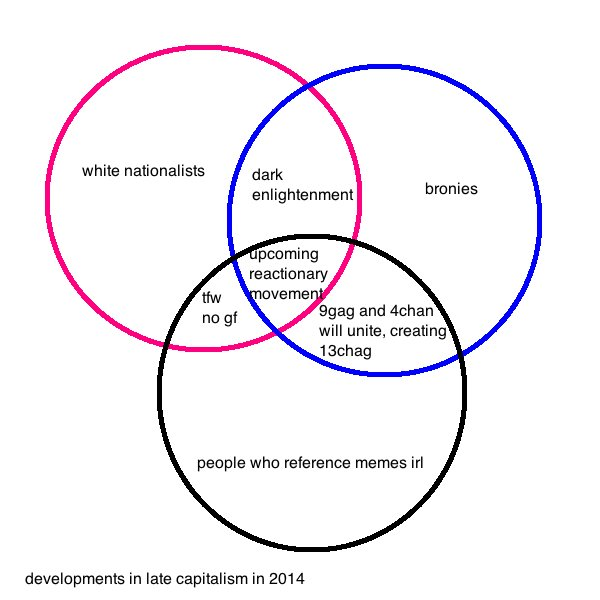
\includegraphics[width=0.7\linewidth]{images/internet-capitalism-2014.png}
  \caption{Desarrollo del capitalismo tardío en 2014, según un foro de internet.}
  \label{fig:capitalism2014}
\end{figure}

Según la derecha alternativa de internet --probablemente los foros más cínicos de estos días-- la izquierda se posiciona como una Catedral dogmática que abraza y reproduce el marxismo cultural posmoderno para planear una guerra, un sabotaje en contra de la civilización occidental. La crítica de los neorreaccionarios al sentimiento religioso-folklórico es que es moralista y es una posición primitivista. La Catedral es el principal centro de resistencia frente a la agenda de productividad del movimiento neorreaccionario. Además de la connotación de dogmatismo religioso, la Catedral también se refiere a la élite progresista de izquierda liberal. Distintos grupos de derecha en internet se dedican a señalar cómo la izquierda se destruye a sí misma a través de la política folk, que identifican con el rechazo a las instituciones y con un activismo micro, local, autocomplaciente.

La Catedral representa la herencia de Occidente y es, por ello, un enemigo del progreso. Los neorreaccionarios toman partido por la utopía tecnocapitalista y consideran a la política como un enemigo para sus fines. La fantasía biónica de Nick Land, cuya posición poshumanista crea una dicotomía entre una superinteligencia antihumanidad y la emancipación universal, yace en el trasfondo de estos proyectos. Singapur y Hong Kong son ejemplos de la utopía pospolítica.

La política folk es una experiencia de la política como droga, como mero entretenimiento, algo que en los foros de internet describen como \emph{choose your own adventure}. Srnicek y Williams la describen como una política afectiva, micro, sin ser efectiva a nivel macro. Ocurre por tres razones:

\begin{itemize}
  \item Incapacidad de lidiar con la complejidad, con el complejo entramado de formas de violencia y de sujeción al poder del capital. Por ejemplo, en los mercados, donde diversos ciclos de producción están relacionados directamente a otras variables y ellas, a su vez, dependen de fenómenos macroeconómicos poco accesibles a la gente común.
  \item Reacción a las instituciones políticas de izquierda tradicionales, a lo que los neorreaccionarios llaman la catedral por un comportamiento sectario centrado en la organización comunitaria. Surge con la decadencia del movimiento hippie y se caracteriza por un vuelco al localismo y horizontalismo \autocite{TyrannyStucturelessness,TyrannyTyranny}. 
  \item Reacción simbólica al espectáculo político. Es decir, frente a la industria de los medios de comunicación, que transforman toda experiencia de vida en representación capitalizable, la política folk decidió evitar cualquier confrontación mediática y de la farándula de la militancia institucionalizada para volcarse al activismo hiper-local que construyera alternativas comunitarias \emph{in-situ}. Esta situación se explica en parte por la disolución de los polos EUA-URSS después de la caída del muro de Berlín.
\end{itemize}

La política folk es un concepto que se refiere a una forma que surge tras la caída de los grandes movimientos hegemónicos y se puede localizar en la época posmoderna como una condición de marginalidad tras la victoria del capital sobre las otras grandes narrativas históricas. Acción directa, democracia real y anti-jerarquía son algunas de las características de esta práctica política. Pareciera que hoy en día sobran tácticas políticas y gestos de desobediencia pero la cuestión sobre cómo crear una alternativa política a escala global o molar sigue abierta y ha sido olvidada por buena parte de la izquierda contemporánea. \emph{Inventar el futuro} aborda esta cuestión con un programa político que denosta la participación folklórica de distintos grupos de izquierda para lanzarse a la exploración de un proyecto económico hegemónico que se lanza a la disputa por el universalismo, el progresismo y otras categorías que forman parte de la herencia de la Ilustración \autocite[p.~14]{srnicekInventarFuturoPoscapitalismo2017}. Si bien es una propuesta coherente al interior del Estado para crear una sociedad poscapitalista, su base sigue dependiendo en la ligadura economía-Estado, por lo que su respuesta al desarrollo voraz del capitalismo sigue siendo occidental. Es decir, presupone que la \emph{forma de vida} por excelencia es la ciudadanía y no atiende realmente a las razones que producen a la economía mercantil como un régimen de deseo.

Pese a que Srnicek y Williams abordan con relativa claridad el fenómeno, no parece ahondar demasiado en la naturaleza psíquica de la sociedad mercantil contemporánea. La política folk es problemática por diversas razones. Una de las más relevantes para este trabajo tiene que ver con cómo lidiar con la complejidad del mundo. Es ahí donde profundizar en la relación entre Estado y economía se vuelve sumamente relevante. La aparente autarquía de los mercados funciona a través de un caótico entramado de transacciones.

La necesidad de coherencia y la invisibilización de los privilegios, lo opuesto a lo que Donna Haraway llamaría \emph{conocimiento situado}, hace que las izquierdas en Estados Unidos caigan en el descrédito mediático a través de falacias argumentativas que hace ver a las personas de izquierda (señaladas en tono irónico como \emph{Social Justice Warriors}) como gente inestable e incoherente en lo que respecta a una agenda política común y popular. En general, los movimientos de izquierda son aplastados mediáticamente a través del cinismo y la ironía. Por esa razón, las estrategias de izquierda tienen que tener en cuenta que lo que caracteriza a las posturas conservadoras, tradicionalistas o reaccionarias, es el \emph{resentimiento}, operado a través de la retórica del cinismo contemporáneo.
 Una alternativa política debe partir del reconocimiento tecnomaterialista y de la estrategia política. En el mismo ensayo, \autocite{huiUnhappyConsciousnessNeoreactionaries2017} señala que la modernidad es más bien la dominación tecnológica que despoja a cualquier forma social de interioridad a través de un proceso de apropiación tecnopolítica. Es decir, la cuestión tecnológica está en el centro del problema político contemporáneo.

La tiranía de la ausencia de estructura es un problema de reconocimiento del deseo. Yo considero que hay algo de cierto en el diagnóstico de las derechas de Estados Unidos con respecto a las dificultades de las izquierdas pero adjudico las causas a un proceso sociológico señalado en \autocite{TyrannyStucturelessness}. Presas de la nostalgia, muchos intelectuales de \emph{ethos} virilista reproducen un dogmatismo y control sectario incluso en los grupos de activistas. Las izquierdas más reconocidas en los medios masivos están compuestas de hombres virilistas de prácticas autocomplacientes que buscan autoridad sobre las demás personas a través del carisma.

\section{La época de la Ilustración es también llamada el siglo de Federico}
\label{sub:la-época-de-ilustración}

\epigraph{\enquote{Igualmente, un sacerdote está obligado a un puesto que fue aceptado bajo esa condición. [\ldots] La Ilustración es la potencia o condición histórica de discernimiento propio en materia de religión}}{\emph{Immanuel Kant} en~\autocite[p.~96]{kantQueEsIlustracion2009}}

La propuesta de Kant le hablaba a los príncipes alemanes como agentes de la Historia universal, pero se volvieron cínicos. La causa es que la crítica en el seno del Estado moderno encarna una contradicción manifiesta en el teatro político de la \emph{publicidad}. Este proceso tiene un equivalente mediático, el periódico. Podemos identificar la religiosidad del proyecto de Estado en la máxima kantiana de la fe en la acción pública. Su pregunta es cómo plantear la fe a través de la acción crítica como la finalidad de la Historia, y en consecuencia, como objeto del Estado. Su respuesta es tan satisfactoria que permite el despliegue y sofisticación de las cortesías y los manuales de etiqueta que caracterizaban a la política monárquica y al teatro de las cortes y los parlamentos europeos.

Paradójicamente, la democracia liberal tiene su génesis en esos procesos y reproduce la lógica de la ciudadanía griega de la pertenencia a la polis, de la capacidad de participar de los asuntos públicos periódicamente.

Federico fue el primer soberano de la pluralidad ética como solución a la guerra de religiones. Acogió a Voltaire y señaló que la tarea del Estado era llevar la ilustración y la cultura hasta el último rincón del mundo. Es decir, se trata de la puesta en operación de un dispositivo de guerra. En la modernidad, la superación y captura tecnológica se convierten en la forma de apropiación del Estado de toda forma de interioridad.

El progreso y el universalismo son conceptos en disputa. Los sentidos de la Ilustración según el artículo de Hui son, por un lado, el de Diderot y por otro el de Hume. Algo parecido a la tensión entre el espíritu estoico y el escéptico de los que habla Hegel. El progreso ha sido malentendido. La modernización se convirtió en una empresa colonial y de esclavitud.

En su \emph{Filosofía de la historia}, Kant plantea una fe para el progreso basada casi en su totalidad en la acción. El filósofo alemán escribió desde un principio para los príncipes que pudieran leerlo con la intención de suscitar en ellos el interés por dar un curso racional e iluminista a la historia a partir de la razón. Su fe en la Historia es también un llamado a la acción para los príncipes. Pero la publicidad de la que habla Kant produce un simulacro. Reproduce la lógica de las cortes como el manual de comportamiento de la vida pública y neutraliza toda forma de violencia, todo conflicto confesional, en un debate cuya plataforma técnica es la escritura y su medio la prensa escrita. En este sentido, la prensa es una consecuencia de la imprenta vernácula y la reafirmación de la escritura como plataforma general de la teoría y de la práctica. El texto se vuelve la unidad de información que permitirá la transición de sociedades soberanas a sociedades disciplinarias.

\epigraph{La operación principal del Estado consiste en transformar todo deseo en deseo de Estado.}{\emph{Gilles Deleuze} en~\autocite{deleuzeMilMesetasCapitalismo2002}.}

El hecho de que la derecha alternativa plantee una posición neomonarquista basada en ideas protofascistas atañe a un proceso histórico nacido en tiempos de la posguerra y es lo que Agamben señala como el estado de excepción, donde el exterminio es la normalidad. La finalidad de los neorreaccionarios es reinstaurar la vieja gloria de la civilización occidental rompiendo con la inercia integradora del proyecto imperial y abogando por una separación entre semejantes ilustrados frente al mundo salvaje. La ironía de estos sujetos expone los arreglos epistémicos de la sociedad poshistórica (y por extensión, posverdad) y expone los defectos de la Ilustración. La cuestión de fondo tiene que ver con la forma como el Estado ha configurado todas las subjetividades y en cómo se instaura a través de la necesidad, transmutando todo deseo en interés. De este modo, el interés es el elemento fundacional de la \emph{societas}. Y el público no es otra cosa que los propietarios argumentando en favor de su posición en el arreglo mercantil.

Para la disputa de los sentidos de la Ilustración, hay que entender para qué opera en realidad el Estado moderno y cómo se vale del discurso de la Ilustración y de la Ciencia para justificar su poder, para crear una religión de sí mismo. Como actitud de fondo al drama contemporáneo, el cinismo surge como instrumentalización de la razón a partir de la distinción entre razón pública y privada. Basta recordar que Kant fue un gran admirador de Federico el Grande, que decía sin reparo \enquote{críticad cuando queráis pero obedeced}. El cinismo consiste en la victoria de la tristeza y de la melancolía. La toma de partido del cínico es una respuesta a la contradicción al preferir la servidumbre de sí mismo a la libertad a partir del reconocimiento del deseo afuera del deseo de Estado.

\section{El neoliberalismo se ha apropiado del futuro}
\label{sec:el-neoliberalismo-se-ha-apropiado-del-futuro}

¿Cómo recuperamos la imaginación política? Mientras que Francis Fukuyama plantea el fin de la guerra de ideas \autocite{fukuyamaFinHistoriaUltimo1992}, Samuel Huntington plantea el choque de civilizaciones tras la victoria de la democracia liberal \autocite{huntingtonClashCivilizationsRemaking1996}. Es entonces cuando comienza la guerra contra el terrorismo y la transición de la posmodernidad a la era digital. Tenemos como ejemplos el \emph{Global Action Day} o el movimiento Antiglobalización como reacciones al proyecto neoliberal. Sin embargo, vivimos en un tiempo donde los mecanismos de poder se vuelven difusos y, en el peor de los casos, \emph{capturables}. Podríamos decir que es el fin del maniqueísmo, pues la ruptura de amenazas exteriores y el vuelco a la política interior y a externalidades de globalización como prioridad de seguridad de los gobiernos mundiales, actúan a través de múltiples registros. En ese sentido, si los Estados-nación veían su política a la \emph{Westfalia}, hoy nos enfrentamos a entidades transnacionales que hacen su propia legislación. En pocas palabras, se trata de otro repliegue del imperio, donde la aceleración de las contradicciones llega hasta un nuevo punto de exterminio: la automatización y, en medio de ello, lo probable de la singularidad \autocite{fraseFourFutures2011,fraseFourFuturesVisions2016}.

La lógica de medios y de instituciones nos condicionan al consumo. Hay que tomar posición sobre el mercado. Durante mi investigación me encontré con la dificultad conceptual de relacionar y ser capaz de diferenciar los conceptos de Estado, mercado y capitalismo. Quería entender cómo se produjeron los discursos que hacen que distintos componentes histórico-políticos dieran forma al estado actual de las cosas. Aprendí que en el neoliberalismo, la ciencia se transforma en el discurso justificador y la sociedad se adapta para ejercer un control más exquisito y perfecto sobre el deseo. Experimentamos aquí una transfiguración del Biopoder en despliegues cibernéticos que desmaterializan los dispositivos de poder, traduciendo las normas en impulsos eléctricos y bioquímicos y reduciendo al capitalismo, cada vez más, al mero flujo y tráfico de información. Este proceso evidencia al Principio, como máscara del Imperio, para desplegar un régimen de normas y dispositivos, para despersonalizar todo poder y para conducirnos a la agonía misma del Estado en el fin de la historia. 1989 es un símbolo de ese proceso. La caída del muro de Berlín anuncia el fin de la historia y el auge devastador de la hegemonía neoliberal revela al Imperio como el aparato patético que tiende a controlar cualquier posible eventualidad.

Muchos hombres activistas de izquierda niegan comportamientos machistas y totalitarios en los movimientos en los que operan. Sin embargo, el conocido artículo \emph{Tyranny of Structurelesness} desarrolla los modos informales de control de las autoridades de facto en las organizaciones y señala el comportamiento virilista como un problema de importancia considerable. Una de las múltiples réplicas a este ensayo, \emph{Tyranny of Tyranny} profundiza en lo costoso del cinismo de aquellos hombres aburridos que Tiqqun denominaría como bloomescos \autocite{TyrannyTyranny}. Su comportamiento reproduce el deseo de Estado a través de la deuda, creando una suerte de impuesto moral por el que las personas activistas se redimen, sin buscar necesariamente acciones estratégicas, como si se tratase de una guerra.

Srnicek y Williams apuntan a la construcción de imaginarios que permitan lidiar con la complejidad del mundo contemporáneo para navegar en un terreno político donde el discurso tecnocientífico y la retórica están al servicio de pensamientos que podríamos agrupar en la categoría de derecha alternativa pero también de nuevas derechas. Cómo crear una masa crítica revolucionaria con poder suficiente como para dar un salto más allá de la cultura de la crisis, del Espectáculo de la catástrofe. Antes de continuar, debemos advertir nuevamente sobre la capacidad del Estado de asimilar otras expresiones y voces, capacidad nos deja sin ninguna posibilidad legítima de hacer frente a él. Ni las protestas interminables ni el terrorismo total ni la socialdemocracia reformista son ahora dignas de considerarse estrategias políticas. La práctica política del futuro es tan difusa como los dispositivos con los que está (des)armándose a cada momento.

Para recuperar la imaginación política hay que entender cómo se produce la imagen en el posfordismo, con la cibernética aumentando la dependencia del humano a la máquina.

Si bien el proceso constituyente por el que abogan propuestas como el populismo de Laclau y Mouffe \autocite{laclauRazonPopulista2016} o la posición de Hardt y Negri \autocite{hardtImperio2005} es clave para la revolución, el elemento transformador (por radical y revolucionario) se encuentra en realidad en el poder destituyente, que es la forma en que se generan resistencias escalables tan efectivas que puedan suplir al capitalismo (y en consecuencia, hacer cada vez menos necesario al Estado). El horizonte ético de este poder destituyente ha sido señalado por Hardt y Negri en Imperio y por el Comité Invisible, en las reflexiones sobre la revolución \autocite{comiteinvisibleAhora2017}. Este consiste, entre otras cosas, en retomar la lucha spinoziana por cultivar potencias para el libre juego de las formas de vida. Claro está que los problemas económicos que habrá que enfrentar para hablar sobre el fin del capitalismo son vastos y complejos, pero para abordarlos haremos una breve disección en los componentes de este modo necropolítico de producción para analizar particularmente los conceptos de mercado, eficiencia y efectividad.

Los zapatistas creen que su planteamiento es más moral porque reivindica la lucha de los de abajo y en ese sentido reafirman al capitalismo como poder dominante y no le pueden quitar el componente simbólico de dominación porque lo reconocen. además, al asumir su papel no se comprometen con hacer del zapatismo un modo de vida para todas las personas porque no ofrecen alternativas reformistas que acerquen a la gente, como el blockchain o la organización descentralizada. Y si lo hacen, no es visible.

En \emph{Four Futures}, Peter Frase propone cuatro escenarios para simplificar las posibilidades políticas que hay para las próximas décadas. A este análisis vale la pena sumar otra cuestión: dentro de las principales estrategias del Estado se encuentran la guerra contra el terrorismo y un régimen económico que, en referencia a Preciado, llamaremos farmacopornista \autocite{preciadoTestoYonqui2008,fraseFourFuturesVisions2016}.

\section{El problema político \emph{real} es la captura tecnológica del deseo}
\label{sec:el-problema-político-real}

\epigraph{(\textsf{Pregunta}) ¿Si pudiera ver un documental sobre un filósofo, sobre Heidegger, Kant o Hegel, qué es lo que querría ver?\\ (\textsf{Respuesta de Derrida}) Que hablen de su vida sexual. ¿Quería una respuesta rápida, no? Su vida sexual.}{\emph{Jacques Derrida} en~\autocite{dickScreenplayEssaysFilm2005}.}

El problema de la Historia de Hegel es su posición idealista y lo que ella dice de la guerra de religiones. La victoria de la forma Estado capitalista es también la tensión entre protestantismo y catolicismo, entre la representación y la iconografía. Sin embargo, además de moverse por el deseo de \emph{ser como}, de encarnar la figura de Cristo, de reproducir la lógica de la representación, las formas de vida actúan pulsionarmente, en un dominio psíquico que, pese a los grandes esfuerzos del Biopoder, permanece oculto, sin que por ello sea no explotable. Somos máquinas deseantes, formas de vida. La explicación de la neorreacción tiene una instancia molar, la de la gran narrativa del Estado, la de un lenguaje para sí que configura lo real en el tiempo y en el ambiente. Sin embargo, hay otra posible explicación a otra nivel molecular, psíquico, que atañe a la respuesta de las formas de vida a los estímulos. Bajo esta explicación, los neorreaccionarios son sujetos frustrados y castrados sexualmente. Configuran la multitud que toma partido por el resentimiento sexual y por una pulsión ---retomando a Preciado--- \emph{snuff}.

El tecnomaterialismo se parece mucho a lo que imagino como cruce entre una forma molar y otra molecular de analizar el poder. En relación con la escasez de recursos, el deterioro y acelerada pauperización son reales. Frente al tecnofascismo se necesita abrir otra vez la cuestión del Partido y eso solo se puede lograr analizando dónde se sitúan los deseos. Mientras que Nick Srnicek y Alex Williams buscan la configuración de un movimiento político de vanguardia, Preciado, retoma el análisis crítico sobre las condiciones tecnopolíticas de dominación y propone una visión del trabajo desde el concepto de \emph{potentia gaudendi} o fuerza orgásmica para entender otras formas de producción de valor en el mercado. Desarrollaré el argumento de que hay una tensión entre la economía como el problema mismo y la economía como condición emancipatoria de la propia economía. Me interesa entender cuáles son los límites tácticos y horizontes que, a partir del mercado, puedan contribuir a una práctica difusa de la política radical, tendiendo siempre como horizonte la potencia común para el libre juego de las formas de vida.

La crisis tiene dos caras: por un lado, la ecocatástrofe producida por el despliegue trasnacional del capital, y por el otro, el cinismo y el nihilismo como síntomas de la crisis de la religión de Estado (o lo que Fukuyama llamaría \enquote{fin de la historia}). No deja de ser claro que, a pesar de lo anterior, la lucha inicia destituyendo el Espectáculo, pero se gana en el terreno de los recursos económicos, por la dificultad de obtener y gestionar bienes y necesidades. Tecnomaterialismo considera los procesos productivos como lo que configura las relaciones sociales. Desde este punto de vista, somos configuradas por las interfaces y el ecosistema que nos produce. El problema de la falsa conciencia ilustrada quizá tiene que ver con una respuesta psíquica colectiva que produce amos y esclavos a través de los flujos de codificación del deseo.

Crítica al optimismo tecnológico: El sueño utópico de marxismos y anarquismos, de un mundo donde la tecnología supondría la emancipación del hombre, es técnicamente posible. Es decir, en la actualidad existen suficientes herramientas no solo para aliviar la pobreza sino para garantizar la libertad efectiva, sintética de acuerdo con Nick Srnicek, para todas las personas en el planeta. Sin embargo, el presente es también el momento de la instauración definitiva de la crisis y de la invisible aceleración de la ecocatástrofe, que silencia las voces de quienes no tienen rostro y las confunde con el ruido transparente de los circuitos de producción de sentido del Imperio. Las consecuencias del fin de la historia no han sido otras que la reafirmación y reconfiguración de la autoridad estatal en dispositivos de poder cada vez más difusos. El síntoma más claro de la crisis está en la crisis de la democracia liberal, que resulta cada vez más rebasada frente a las distintas subjetividades y a la cuestión tecnológica ---que está directamente relacionada con el trabajo.

Todo pensamiento es estratégico en la medida en que el problema político contemporáneo es el entramado de tecnologías que producen los dispositivos de la cibernética. Thiels, uno de los inversionistas ángel más aclamados de Sillicon Valley, es una muestra de esto. Parte de una experiencia, de un \emph{pathos}, parecido al de Spengler. En la visión de este teórico podemos encontrar una experiencia muy semejante a lo que Tiqqun describe como el Bloom. La Ilustración oscura\footnote{Traducción nuestra para referirnos al concepto de Dark Enlightenment de Nick Land, del que parten los neorreaccionarios para fundamentar sus posturas. \autocite{DarkEnlightenmentNick2012} parte de una oposición entre libertad y democracia \autocite[p.~5]{huiUnhappyConsciousnessNeoreactionaries2017}}. Lo que se oculta detrás de su posición es una vaguedad conceptual en la que se considera como democracia a la simulación representativa electoral que da forma a la mayoría de los Estados-nación contemporáneos.

El resentimiento es el sentimiento principal de los neorreaccionarios. ¿Por qué es preocupante este resentimiento? Simplemente porque este sentir contagia a formas de vida que acumula agencia tecnomaterial. Es decir, capacidad para transformar la realidad. Lo que significa que de los cuatro escenarios posibles para un futuro cercano, este grupo probablemente decida de hecho hacia qué camino transitan las sociedades en su conjunto.

En la actualidad, el descontento por la \enquote{democracia liberal} es parte de una disputa más profunda sobre el progreso, la democracia y el universalismo. La corriente neorreaccionaria es una de las más férreas opositoras a la democracia liberal y es quizá aquí donde tengan un punto de comunión con diversas posiciones políticas que también se le oponen. Sin embargo, es necesario recordar que la alternativa para los neorreaccionarios no es otra sino una utopía tecnototalitaria ciudadanista.

\begin{table}[htb]
  \caption{Escenarios planteados en \emph{Four Futures} respecto al porvenir global.}
  \label{tab:ubicua}
  \centering

  \begin{tabular}{ccc}
    \toprule
    & \textbf{Abundancia} & \textbf{Escasez}\\
    \midrule
    \textbf{Igualdad} & Comunismo & Socialismo\\
    \textbf{Jerarquía} & Rentismo & Exterminismo\\
    \bottomrule
  \end{tabular}
\end{table}

El problema político es un imaginario del futuro que nos lleve al escenario ideal en \emph{Four Futures} El problema de acción es la tiranía de la ausencia de estructura. En realidad este fenómeno se da porque es realmente complicado hacer una alternativa que ataque diferentes violencias transversalmente. La falta de estructura se explica como un arreglo económico sobre el deseo donde prevalece la mala conciencia, el resentimiento y latencias de un orden jerarquizado y estamentario (unión con precariedad-jerarquía de \emph{Four Futures}.

Una de las cuestiones que más ocupa a Fraser es la cuestión de cómo podría darse un escenario de comunismo real si las clases de personas ricas y propietarias opondrán resistencia de forma violenta a cualquier insurrección. Para Tiqqun, la guerra civil es el libre juego de las formas de vida, el principio de su coexistencia. Las sociedades tradicionales conocían el robo, la blasfemia, el parricidio, el rapto, el sacrificio, la afrenta y la venganza. Por otro lado, las sociedades modernas se apropian de la capacidad de decidir sobre cualquier conflicto social. La violencia es aquello de lo que hemos sido desposeídos, y aquello de lo que hace falta ahora reapropiarse.

El Estado es una religión que captura nuestro deseo y lo incorpora al contrato social. Un movimiento real debe permitir a las personas ser agentes de su deseo. Por eso la ciudadanía no resuelve nada, es deseo de deseo de Estado. En el deseo de Estado manifiesto religiosamente a través del trabajo, perviven latencias de sociedades premodernas adaptadas a un mito que adapta las jerarquías tradicionales y la obediencia al desarrollo de las formas de producción de valor de las mercancías. La religión de Estado transforma deseo en interés. el cinismo es el dispositivo discursivo que produce placer a quien se congratula de su impotencia, de instrumentalizar la crítica.

Históricamente, la gestación del Estado moderno se sitúa en la guerra de religiones como contexto histórico de la guerra civil en la sociedad tradicional y recuerda un poco a la reflexión de Hegel sobre el judaísmo y el cristianismo en la Historia de la conciencia absoluta. La impronta ética de las visiones afuera del Estado moderno hoy en día, no son capaces de plantear una totalidad plena de sentido, un sentimiento de universalidad. Mientras, la neorreaccion hoy en día consiste en la construcción de intenciones racionalistas y bajo el discurso tecnocientífico, de una utopía tecnocapitalista cuyos exponentes máximos son Hong Kong y Singapur. Para mí, este fenómeno muestra dos caras de un profundo proceso de alienación que tiene que ver con la correcta asimilación parasitaria del capitalismo al Estado moderno. En el siguiente capítulo analizaremos al Estado operar como entidad tecnológica tanto en un sentido tecnomaterial como en uno libidinal a través de la religión.